\documentclass[10pt]{article}
\usepackage[T1]{fontenc}
\usepackage{lmodern,amsmath,amssymb,graphicx,hyperref}
\usepackage[margin=.75in]{geometry}
\setlength{\parindent}{0pt}\setlength{\parskip}{6pt}
\begin{document}
\begin{center}{\Large A helper outside the actual curve ideal}\\[4pt]
23 November 2026 --- local unsigned Lean evidence\end{center}
\textbf{Setting and endpoint.}
Let $K$ be a field, $2\ne0$, $\deg f\le3$, and $F=Y^2-f(X)$.
Let $S\subset K$ have three elements, with an explicit equivalence
$e:\operatorname{Fin}(3)\simeq S$. Require $x_t\notin S$, $y_t\ne0$,
$z(s)\ne0$, $y_t^2=f(x_t)$ and $z(s)^2=f(s)$ for every $s\in S$.
The actual interpolation operator has 72 coefficient coordinates and 70
mixed-jet rows. Its kernel contains a vector $v$ such that the actual
monic curve remainder of its embedded polynomial $E(v)$ is nonzero.
No favorable rank or remainder witness is supplied [pcc:unverified].

The resulting $p=E(v)$ satisfies
\[
 \deg_Yp\le7,\qquad \deg_Xp_j+2j<16\quad(j\le\deg_Yp),
\]
and full mixed Taylor multiplicity four at $(x_t,y_t)$ and at both
$(s,\pm z(s))$ for all $s\in S$. The coefficient mask is exactly the
original $i+2j<16$ mask. This is fixed-support existence [pcc:unverified].

\begin{center}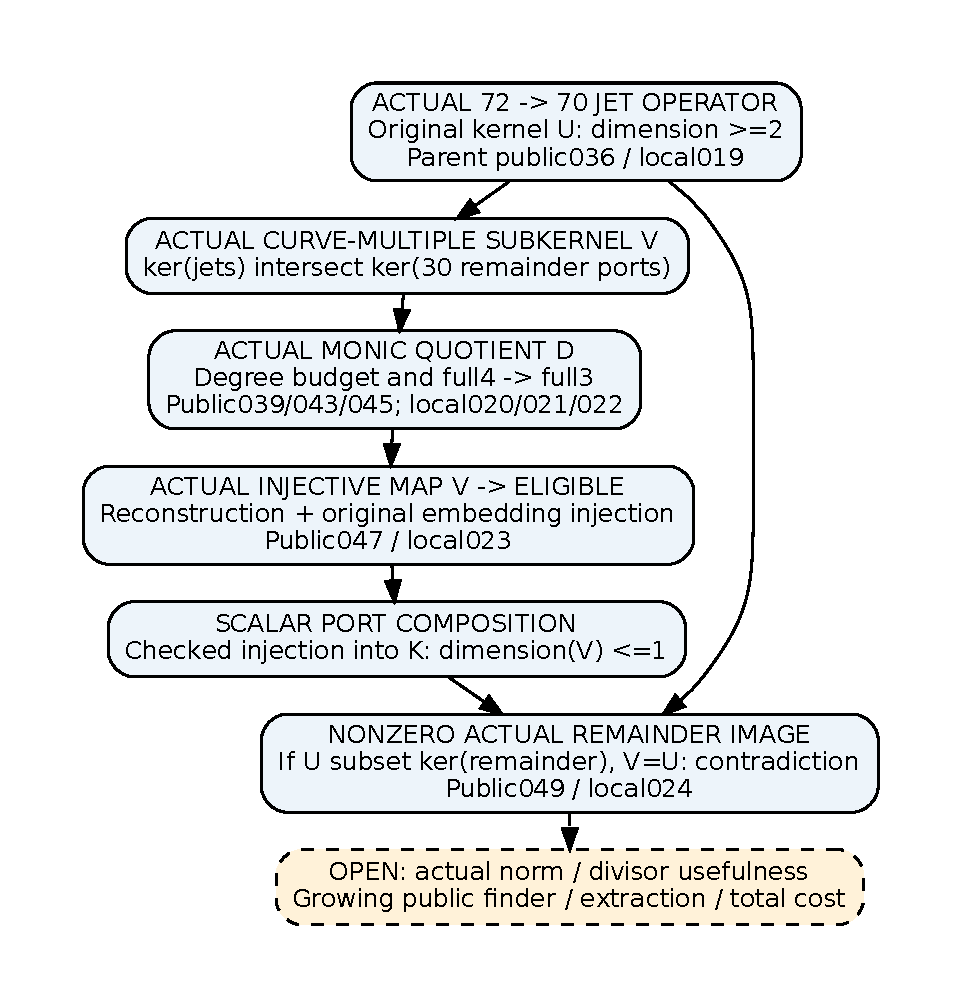
\includegraphics[width=.86\linewidth,height=.58\textheight,keepaspectratio]{noncurve-dependencies-001.pdf}\end{center}
\textbf{Evidence.} Public049/build052/local024, PCC-20261123-80eef0;
126 primary statements including 108 committed parent and 18 new.
Exit zero, no warnings, all printed dependencies standard. These are
unsigned data, outside shared Transport53/57 audit/fresh [pcc:unverified].
\newpage
\begin{center}{\Large The actual quotient bridge}\end{center}
\textbf{Degree, not a supplied budget.}
Write $q_j=[Y^j]E(v)$. The constructed quotient $D=E(v)/_mF$ has rows
\[
\begin{array}{ll}
 D_0=q_2+q_4f+q_6f^2,&D_1=q_3+q_5f+q_7f^2,\\
 D_2=q_4+q_6f,&D_3=q_5+q_7f,\\
 D_4=q_6,&D_5=q_7.
\end{array}
\]
From the original coefficient mask and $\deg f\le3$, the proof derives
$\deg D_j<12-2j$, $\deg_YD<6$. Thus $D$ belongs to the actual
\texttt{budgetSpace}; it is not an assumed strict-budget witness
(PCC-20261123-17efe0) [pcc:unverified].

\textbf{Actual local multiplicity.}
The generic mixed Taylor product formula is separately implemented in the
owning library. The consumer binds its old jet definition to that exact
formula (PCC-20261123-01402a). At an actual curve point, the translated
curve factor has constant coefficient zero and $Y$ coefficient $2y\ne0$.
Its product coefficients at $(0,1),(0,2),(1,1),(0,3),(1,2),(2,1)$
successively force
\[
 D_{00}=D_{01}=D_{10}=D_{02}=D_{11}=D_{20}=0.
\]
These are exactly the multiplicity-three triangle. There is no factorial
division and no assertion that reduction modulo $F$ preserves ambient
jets (PCC-20261123-93790c) [pcc:unverified].

\textbf{Actual linear map and injection.}
Set $U=\ker(\text{original jet map})$ and
$V=U\cap\ker(\text{actual finite remainder})$.
On $V$, monic division gives $E(v)=FD(v)$, so the quotient satisfies
both the degree constraints and actual third jets at the same nodes.
The equivalence $e$ binds the original tuple indices to the actual set.
Equal quotients give equal embeddings by reconstruction, hence equal
vectors by the original coefficient embedding injection.
The constructed map $V\to\text{eligible}$ is therefore injective.
Composing the previously checked scalar port into $K$ gives
$\dim_KV\le1$ (PCC-20261123-9c7116) [pcc:unverified].

\textbf{Nonzero curve image.}
The parent rank-nullity proof gives $\dim_KU\ge2$.
If the actual remainder vanished on all of $U$, then
$U\le\ker(\text{remainder})$, so $V=U$.
The actual submodule equality contradicts $2\le\dim_KU\le1$.
This proves the endpoint, rather than inferring rank from the 30-port
capacity (PCC-20261123-80eef0) [pcc:unverified].
\newpage
\begin{center}{\Large Reproducible evidence and next discriminator}\end{center}
\textbf{Proof map.} Namespace prefix \texttt{Orientation} is omitted below.
\small
\begin{tabular}{p{.23\linewidth}p{.48\linewidth}p{.2\linewidth}}
Source/build/receipt & Main declarations & New/total\\\hline
039/040/020 & ActualQuotientBudget.actual\_quotient, curveQuotient\_mem\_budgetSpace &7/115\\
043/046/021 & OwnerMixedBinding.owner\_mixed\_eq\_actual, fullMultiplicity\_owner\_iff &3/118\\
045/048/022 & CurveLocalTransport.curve\_mixed\_coefficient, curve\_full\_four\_to\_three &2/120\\
047/050/023 & ActualSubkernel.quotient\_mem\_eligible, quotientToEligible\_injective, curveSubkernel\_finrank\_le\_one &4/124\\
049/052/024 & NonzeroRemainderImage.nonzero\_remainder\_image, actual\_noncurve\_helper &2/126
\end{tabular}
\normalsize

\textbf{Dependency scope.}
Lean4.35.0 and Mathlib revision
\texttt{cfc55fc58714a59dc06e6e79edc6d1d95140d3c2} are pinned.
Separate owner commit \texttt{cbc661ca43cc5421ae1db6bf9cb7dc0939ff22a0}
adds \texttt{CryptoLean.PolynomialMixedTaylor}: four generic CommSemiring
statements, focused module build, existing audit four passed/zero
extra trusted axioms. The consumer uses an explicit 45-file compiled
overlay; old modules are not replaced. Primary manifests, umbrella and
shared gates are unchanged. No whole-project/fresh or signed standing
is inferred [pcc:unverified].

\textbf{Failures retained.}
Failed source037 and unlaunched038 retain original bytes.
Precall041 had stale administrative metadata and was never launched.
Build042 failed at import namespace composition; an explicit pinned
overlay corrected it. Builds043--045 rejected public coercion forms.
Build047 rejected Taylor/constant simplification and cancellation scripts;
049 rejected a map-value normal form. Build051 has one deprecated-tactic
warning;052 uses the supported tactic without suppression.
Every source/raw log/exit and all previous report snapshots are retained.
No builds039 or041 were launched.

\textbf{Sources and interpretation.}
Reuse actual Mathlib Taylor, coefficient, monic-division and dimension
laws and the separately audited owner module. The earlier primary
\href{https://doi.org/10.1109/TIT.2013.2243800}{Beelen et al.2013,
SectionIII/Theorem6/(2)} review supplies the interpolation comparator;
its sufficient count does not become an existence theorem by assumption.
The research-KB MCP is not loaded and its wrapper has no executable.
No novelty claim is made for standard interpolation or Taylor algebra.

\textbf{Next discriminating proof.}
For actual $A=\operatorname{evenPart}(f,v)$,
$B=\operatorname{oddPart}(f,v)$ and actual cubic $f$, prove
$N=A^2-fB^2\ne0$ from the established nonzero remainder and odd degree,
then $\deg N\le30$ [pcc:unverified]. Next prove actual norm root orders and divisor/scalar
content. Do not assume residual splitting, useful factor-base support,
independent relations or free preparation. Growing-support public finding,
coverage/retry, extraction and full expected bit cost remain open.
The original nonscalar origin and rank-directed $W$-jet mechanisms are
separate open bridges. Protected remote PCC divergence prevents push;
no ledger reconciliation, signing or gate bypass was attempted.
\end{document}
